%% AMS-LaTeX Created with the Wolfram Language : www.wolfram.com

\documentclass{article}
\usepackage{amsmath, amssymb, graphics, setspace}

\newcommand{\mathsym}[1]{{}}
\newcommand{\unicode}[1]{{}}

\newcounter{mathematicapage}
\begin{document}

\section*{Modelling Practice --$\unicode{5bf9}\unicode{4e8e}\unicode{52a8}\unicode{7269}\unicode{4f53}\unicode{91cd}\unicode{548c}\unicode{5fc3}\unicode{7387}\unicode{5173}\unicode{7cfb}\unicode{7684}\unicode{5efa}\unicode{6a21}$}

\subsection*{$\unicode{5efa}\unicode{6a21}\unicode{5047}\unicode{8bbe}$ Assumption$\unicode{ff1a}$}

1. $\unicode{54fa}\unicode{4e73}\unicode{52a8}\unicode{7269}\unicode{8eab}\unicode{4f53}\unicode{5316}\unicode{5b66}\unicode{6210}\unicode{5206}\unicode{76f8}\unicode{4f3c}\unicode{ff0c}\unicode{5373}\unicode{5bc6}\unicode{5ea6}\rho
\unicode{76f8}\unicode{540c}\unicode{3002}$

2. $\unicode{5355}\unicode{4f4d}\unicode{65f6}\unicode{95f4}\unicode{6563}\unicode{5931}\unicode{70ed}\unicode{91cf}\unicode{4e0e}\unicode{8be5}\unicode{7269}\unicode{79cd}\unicode{76ae}\unicode{80a4}\unicode{9762}\unicode{79ef}\unicode{6210}\unicode{6b63}\unicode{6bd4}\unicode{ff0c}$Q
$\propto $ S$\unicode{3002}$

3. $\unicode{54fa}\unicode{4e73}\unicode{52a8}\unicode{7269}\unicode{5fc3}\unicode{5ba4}\unicode{5bb9}\unicode{79ef}\unicode{548c}\unicode{8be5}\unicode{54fa}\unicode{4e73}\unicode{52a8}\unicode{7269}\unicode{4f53}\unicode{79ef}\unicode{6210}\unicode{6b63}\unicode{6bd4}\unicode{ff0c}\unicode{5373}$
\(V_0\) $\propto $ V$\unicode{3002}$

4. $\unicode{5355}\unicode{4f4d}\unicode{4f53}\unicode{79ef}\unicode{8840}\unicode{6db2}\unicode{643a}\unicode{5e26}\unicode{80fd}\unicode{91cf}\unicode{76f8}\unicode{540c}\unicode{ff0c}\unicode{4e3a}$
D$\unicode{3002}$

\subsection*{$\unicode{6a21}\unicode{578b}\unicode{5efa}\unicode{7acb}$ Construction$\unicode{ff1a}$}

$\unicode{9996}\unicode{5148}\unicode{ff0c}$W=$\rho $V$\unicode{ff0c}\unicode{5bf9}\unicode{4e8e}\unicode{6240}\unicode{6709}\unicode{7269}\unicode{79cd}\unicode{ff0c}\unicode{8be5}\unicode{79cd}\unicode{52a8}\unicode{7269}\unicode{4f53}\unicode{91cd}\unicode{4e3a}\unicode{8be5}\unicode{79cd}\unicode{52a8}\unicode{7269}\unicode{8eab}\unicode{4f53}\unicode{5bc6}\unicode{5ea6}\unicode{548c}\unicode{4f53}\unicode{79ef}\unicode{7684}\unicode{4e58}\unicode{79ef}\unicode{3002}$\\
$\unicode{8bbe}\unicode{5b58}\unicode{5728}\unicode{67d0}\unicode{4e00}\unicode{7ebf}\unicode{5ea6}$r$\unicode{63cf}\unicode{8ff0}\unicode{8be5}\unicode{79cd}\unicode{52a8}\unicode{7269}\unicode{5927}\unicode{5c0f}\unicode{ff0c}\unicode{5219}\unicode{5e94}\unicode{6709}$
V $\propto $ \(r^3\)$\unicode{ff0c}$S $\propto $ \(r^2\)$\unicode{3002}\unicode{5355}\unicode{4f4d}\unicode{65f6}\unicode{95f4}\unicode{6563}\unicode{5931}\unicode{70ed}\unicode{91cf}\unicode{4e0e}\unicode{8be5}\unicode{7269}\unicode{79cd}\unicode{76ae}\unicode{80a4}\unicode{9762}\unicode{79ef}\unicode{6210}\unicode{6b63}\unicode{6bd4}\unicode{ff0c}\unicode{5373}$
Q $\propto $ S$\unicode{3002}$\\
$\unicode{5355}\unicode{4f4d}\unicode{65f6}\unicode{95f4}\unicode{6563}\unicode{70ed}\unicode{91cf}\unicode{548c}\unicode{7b49}\unicode{4e8e}\unicode{5355}\unicode{4f4d}\unicode{65f6}\unicode{95f4}\unicode{901a}\unicode{8fc7}\unicode{8be5}\unicode{79cd}\unicode{52a8}\unicode{7269}\unicode{8868}\unicode{9762}\unicode{76ae}\unicode{80a4}\unicode{7684}\unicode{8840}\unicode{6d41}\unicode{91cf}$
$\delta $ $\unicode{4e0e}\unicode{5355}\unicode{4f4d}\unicode{4f53}\unicode{79ef}\unicode{8840}\unicode{6db2}\unicode{643a}\unicode{5e26}\unicode{80fd}\unicode{91cf}$D$\unicode{4e4b}\unicode{79ef}\unicode{ff0c}\unicode{5373}$
Q = $\delta $ D$\unicode{3002}\unicode{800c}\unicode{8840}\unicode{6d41}\unicode{91cf}\unicode{7b49}\unicode{4e8e}\unicode{5fc3}\unicode{8df3}\unicode{9891}\unicode{7387}$
n $\unicode{548c}\unicode{6bcf}\unicode{6b21}\unicode{5fc3}\unicode{8df3}\unicode{6cf5}\unicode{8840}\unicode{4f53}\unicode{79ef}\unicode{5373}\unicode{5fc3}\unicode{5ba4}\unicode{4f53}\unicode{79ef}$
\(V_0\) $\unicode{7684}\unicode{4e58}\unicode{79ef}\unicode{ff0c}\delta $ = \(V_0\) n$\unicode{3002}$\\
$\unicode{7531}\unicode{4e0a}\unicode{8ff0}\unicode{5173}\unicode{7cfb}\unicode{53ef}\unicode{63a8}\unicode{51fa}$ n W $\propto $ S$\unicode{ff0c}\unicode{5373}$
n \(W^{\frac{1}{3}}\) = C$\unicode{ff0c}\unicode{5176}\unicode{4e2d}$C$\unicode{4e3a}\unicode{67d0}\unicode{4e00}\unicode{5e38}\unicode{6570}\unicode{3002}$\\


\subsection*{$\unicode{6a21}\unicode{578b}\unicode{6c42}\unicode{89e3}$ Solution$\unicode{ff1a}$}

\begin{doublespace}
\noindent\(\pmb{\text{weights} = \{25,200,2000,5000,30000,50000,70000,450000\};}\\
\pmb{\text{rates} = \{670,420,205,120,85,70,72,38\};}\\
\pmb{\text{products} = \text{weights}^{\frac{1}{3}}*\text{rates};}\)
\end{doublespace}

$\unicode{4e0b}\unicode{56fe}\unicode{4e3a}\unicode{5e38}\unicode{6570}$C$\unicode{968f}\unicode{4e0d}\unicode{540c}\unicode{7269}\unicode{79cd}\unicode{7684}\unicode{53d8}\unicode{5316}\unicode{60c5}\unicode{51b5}$

\begin{doublespace}
\noindent\(\pmb{\text{ListPlot}[\text{products},\text{Joined}\to \text{True},\text{PlotMarkers}\to \text{Automatic},\text{PlotRange}\to \{\{0,9\},\{0,3000\}\},}\\
\pmb{\text{PlotLabel}\to \text{{``}Constant C with different spieces{''}},\text{AxesLabel}\to \{\text{{``}Spicies{''}},\text{{``}Product{''}}\},}\\
\pmb{\text{LabelStyle}\to \{\text{FontFamily}\to \text{{``}Microsoft YaHei UI{''}},\text{GrayLevel}[0],\text{Italic}\},\text{ImageSize}\to \text{Large}]}\)
\end{doublespace}

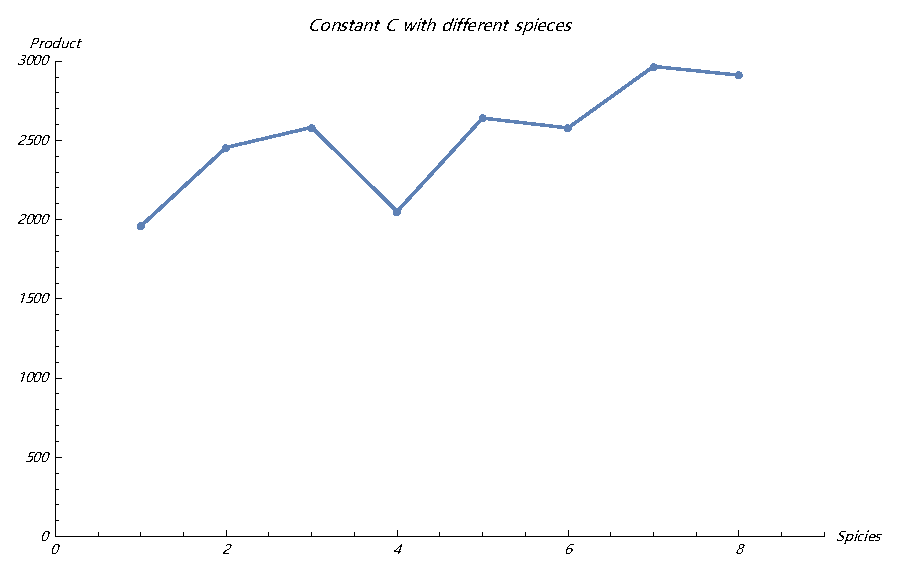
\includegraphics{Modelling Practice_gr1.eps}

$\unicode{4e0b}\unicode{56fe}\unicode{4e3a}\unicode{5e38}\unicode{6570}$C$\unicode{7684}\unicode{5bf9}\unicode{6570}\unicode{968f}\unicode{4e0d}\unicode{540c}\unicode{7269}\unicode{79cd}\unicode{7684}\unicode{53d8}\unicode{5316}\unicode{60c5}\unicode{51b5}$

\begin{doublespace}
\noindent\(\pmb{\text{ListPlot}[\text{Log}[\text{products}],\text{Joined}\to \text{True},\text{PlotMarkers}\to \text{Automatic},\text{PlotRange}\to
\{\{0,9\},\{0,10\}\},}\\
\pmb{\text{PlotLabel}\to \text{{``}Constant C with different spieces{''}},\text{AxesLabel}\to \{\text{{``}Spicies{''}},\text{{``}Product{''}}\},}\\
\pmb{\text{LabelStyle}\to \{\text{FontFamily}\to \text{{``}Microsoft YaHei UI{''}},\text{GrayLevel}[0],\text{Italic}\},\text{ImageSize}\to \text{Large}]}\)
\end{doublespace}

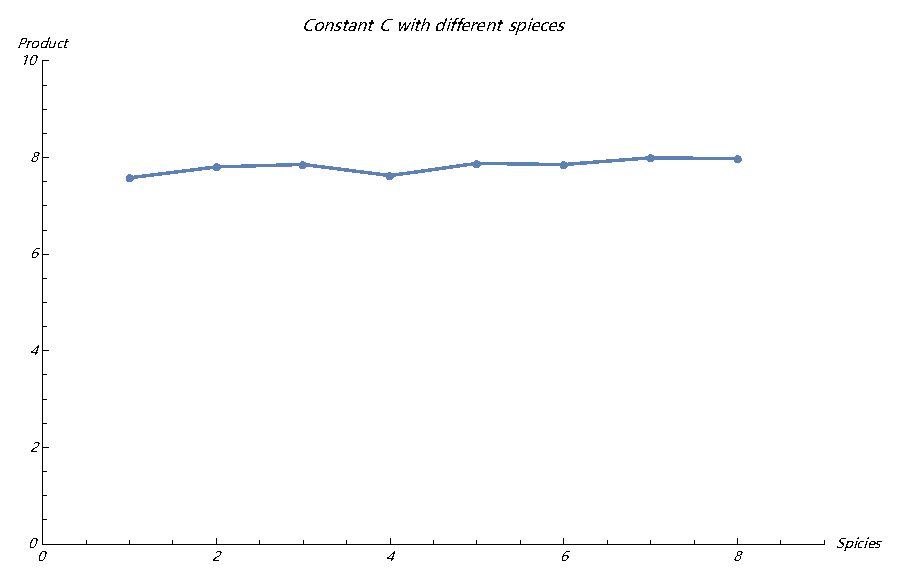
\includegraphics{Modelling Practice_gr2.eps}

\subsection*{$\unicode{6a21}\unicode{578b}\unicode{68c0}\unicode{9a8c}$ Validation$\unicode{ff1a}$}

\begin{doublespace}
\noindent\(\pmb{N[\text{Mean}[\text{products}]]}\)
\end{doublespace}

\begin{doublespace}
\noindent\(2518.67\)
\end{doublespace}

\begin{doublespace}
\noindent\(\pmb{N[\text{StandardDeviation}[\text{products}]]}\)
\end{doublespace}

\begin{doublespace}
\noindent\(361.259\)
\end{doublespace}

\begin{doublespace}
\noindent\(\pmb{\text{Plot}[\text{PDF}[\text{NormalDistribution}[\text{$\%$81},\text{$\%$82}],x],\{x,0,5000\},\text{PlotRange}\to \text{All},\text{ColorFunction}\to
\text{{``}Rainbow{''}}]}\)
\end{doublespace}

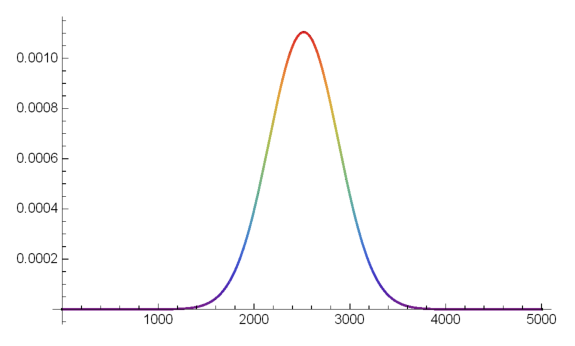
\includegraphics{Modelling Practice_gr3.eps}

$\unicode{6a21}\unicode{578b}\unicode{8f83}\unicode{4e3a}\unicode{7c97}\unicode{7cd9}\unicode{ff0c}\unicode{4f46}\unicode{662f}\unicode{603b}\unicode{4f53}\unicode{6b63}\unicode{786e}\unicode{53cd}\unicode{6620}\unicode{4e86}\unicode{53d8}\unicode{91cf}\unicode{7684}\unicode{5173}\unicode{7cfb}\unicode{3002}\unicode{5176}\unicode{6807}\unicode{51c6}\unicode{5dee}\unicode{4e0e}\unicode{5e73}\unicode{5747}\unicode{503c}\unicode{6bd4}\unicode{503c}\unicode{8f83}\unicode{5927}\unicode{ff0c}\unicode{53ef}\unicode{9760}\unicode{7a0b}\unicode{5ea6}\unicode{4f4e}\unicode{3002}\unicode{9700}\unicode{8981}\unicode{8fdb}\unicode{4e00}\unicode{6b65}\unicode{5b8c}\unicode{5584}\unicode{3002}$

\end{document}
